\documentclass[
  shownotes,
  xcolor={svgnames},
  hyperref={colorlinks,citecolor=DarkBlue,linkcolor=andesred,urlcolor=DarkBlue}
  , aspectratio=169]{beamer}
\usepackage{animate}
\usepackage{amsmath}
\usepackage{amsfonts}
\usepackage{amssymb}
\usepackage{pifont}
\usepackage{mathpazo}
%\usepackage{xcolor}
\usepackage{multimedia}
\usepackage{fancybox}
\usepackage[para]{threeparttable}
\usepackage{multirow}
\setcounter{MaxMatrixCols}{30}
\usepackage{subcaption}
\usepackage{graphicx}
\usepackage{lscape}
\usepackage[compatibility=false,font=small]{caption}
\usepackage{booktabs}
\usepackage{ragged2e}
\usepackage{chronosys}
\usepackage{appendixnumberbeamer}
\usepackage{animate}
\setbeamertemplate{caption}[numbered]
\usepackage{color}
%\usepackage{times}
\usepackage{tikz}
\usepackage{comment} %to comment
%% BibTeX settings
\usepackage{natbib}
\bibliographystyle{apalike}
\bibpunct{(}{)}{,}{a}{,}{,}
\setbeamertemplate{bibliography item}{[\theenumiv]}

% Defines columns for bespoke tables
\usepackage{array}
\newcolumntype{L}[1]{>{\raggedright\let\newline\\\arraybackslash\hspace{0pt}}m{#1}}
\newcolumntype{C}[1]{>{\centering\let\newline\\\arraybackslash\hspace{0pt}}m{#1}}
\newcolumntype{R}[1]{>{\raggedleft\let\newline\\\arraybackslash\hspace{0pt}}m{#1}}


\usepackage{xfrac}


\usepackage{multicol}
\setlength{\columnsep}{0.5cm}

% Theme and colors
\usetheme{Boadilla}

% I define a custom pallete
\definecolor{andesred}{HTML}{1B175E}
\definecolor{andesyellow}{HTML}{ffff00}

% Other options
\providecommand{\U}[1]{\protect\rule{.1in}{.1in}}
\usefonttheme{serif}
\setbeamertemplate{itemize items}[default]
\setbeamertemplate{enumerate items}[square]
\setbeamertemplate{section in toc}[circle]


\definecolor{mybackground}{HTML}{1B175E}
\definecolor{myforeground}{HTML}{0000A0}

\setbeamercolor{normal text}{fg=black,bg=white}
\setbeamercolor{alerted text}{fg=andesred}
\setbeamercolor{example text}{fg=black}

\setbeamercolor{background canvas}{fg=myforeground, bg=white}
\setbeamercolor{background}{fg=myforeground, bg=mybackground}
\setbeamercolor{palette tertiary}{fg=myforeground,bg=mybackground}

\setbeamercolor{palette primary}{fg=black, bg=white}
\setbeamercolor{palette secondary}{fg=black, bg=white!10!andesyellow}
\setbeamercolor{palette tertiary}{fg=black, bg=white}


\setbeamercolor{frametitle}{fg=black}
\setbeamercolor{title}{fg=black}
\setbeamercolor{block title}{fg=andesred}
\setbeamercolor{itemize item}{fg=andesred}
\setbeamercolor{itemize subitem}{fg=andesred}
\setbeamercolor{itemize subsubitem}{fg=andesred}
\setbeamercolor{enumerate item}{fg=andesred}
\setbeamercolor{item projected}{bg=gray!30!white,fg=andesred}
\setbeamercolor{enumerate subitem}{fg=andesred}
\setbeamercolor{section number projected}{bg=gray!30!white,fg=andesred}
\setbeamercolor{section in toc}{fg=andesred}
\setbeamercolor{caption name}{fg=andesred}
\setbeamercolor{button}{bg=gray!30!white,fg=andesred}
\setbeamercolor{title in head/foot}{fg=andesred}



\usepackage{fancyvrb}
\newcommand{\VerbBar}{|}
\newcommand{\VERB}{\Verb[commandchars=\\\{\}]}
\DefineVerbatimEnvironment{Highlighting}{Verbatim}{commandchars=\\\{\}}
% Add ',fontsize=\small' for more characters per line
\usepackage{framed}
\definecolor{shadecolor}{RGB}{248,248,248}
\newenvironment{Shaded}{\begin{snugshade}}{\end{snugshade}}
\newcommand{\AlertTok}[1]{\textcolor[rgb]{0.94,0.16,0.16}{#1}}
\newcommand{\AnnotationTok}[1]{\textcolor[rgb]{0.56,0.35,0.01}{\textbf{\textit{#1}}}}
\newcommand{\AttributeTok}[1]{\textcolor[rgb]{0.77,0.63,0.00}{#1}}
\newcommand{\BaseNTok}[1]{\textcolor[rgb]{0.00,0.00,0.81}{#1}}
\newcommand{\BuiltInTok}[1]{#1}
\newcommand{\CharTok}[1]{\textcolor[rgb]{0.31,0.60,0.02}{#1}}
\newcommand{\CommentTok}[1]{\textcolor[rgb]{0.56,0.35,0.01}{\textit{#1}}}
\newcommand{\CommentVarTok}[1]{\textcolor[rgb]{0.56,0.35,0.01}{\textbf{\textit{#1}}}}
\newcommand{\ConstantTok}[1]{\textcolor[rgb]{0.00,0.00,0.00}{#1}}
\newcommand{\ControlFlowTok}[1]{\textcolor[rgb]{0.13,0.29,0.53}{\textbf{#1}}}
\newcommand{\DataTypeTok}[1]{\textcolor[rgb]{0.13,0.29,0.53}{#1}}
\newcommand{\DecValTok}[1]{\textcolor[rgb]{0.00,0.00,0.81}{#1}}
\newcommand{\DocumentationTok}[1]{\textcolor[rgb]{0.56,0.35,0.01}{\textbf{\textit{#1}}}}
\newcommand{\ErrorTok}[1]{\textcolor[rgb]{0.64,0.00,0.00}{\textbf{#1}}}
\newcommand{\ExtensionTok}[1]{#1}
\newcommand{\FloatTok}[1]{\textcolor[rgb]{0.00,0.00,0.81}{#1}}
\newcommand{\FunctionTok}[1]{\textcolor[rgb]{0.00,0.00,0.00}{#1}}
\newcommand{\ImportTok}[1]{#1}
\newcommand{\InformationTok}[1]{\textcolor[rgb]{0.56,0.35,0.01}{\textbf{\textit{#1}}}}
\newcommand{\KeywordTok}[1]{\textcolor[rgb]{0.13,0.29,0.53}{\textbf{#1}}}
\newcommand{\NormalTok}[1]{#1}
\newcommand{\OperatorTok}[1]{\textcolor[rgb]{0.81,0.36,0.00}{\textbf{#1}}}
\newcommand{\OtherTok}[1]{\textcolor[rgb]{0.56,0.35,0.01}{#1}}
\newcommand{\PreprocessorTok}[1]{\textcolor[rgb]{0.56,0.35,0.01}{\textit{#1}}}
\newcommand{\RegionMarkerTok}[1]{#1}
\newcommand{\SpecialCharTok}[1]{\textcolor[rgb]{0.00,0.00,0.00}{#1}}
\newcommand{\SpecialStringTok}[1]{\textcolor[rgb]{0.31,0.60,0.02}{#1}}
\newcommand{\StringTok}[1]{\textcolor[rgb]{0.31,0.60,0.02}{#1}}
\newcommand{\VariableTok}[1]{\textcolor[rgb]{0.00,0.00,0.00}{#1}}
\newcommand{\VerbatimStringTok}[1]{\textcolor[rgb]{0.31,0.60,0.02}{#1}}
\newcommand{\WarningTok}[1]{\textcolor[rgb]{0.56,0.35,0.01}{\textbf{\textit{#1}}}}
\usepackage{graphicx}
\makeatletter

\makeatother






%%%%%%%%%%%%%%% BEGINS DOCUMENT %%%%%%%%%%%%%%%%%%

\AtBeginSection[]
{
    \begin{frame}
        \frametitle{Agenda}
        \tableofcontents[currentsection]
    \end{frame}
}

\begin{document}

\title{Resampling Methods for Uncertainty}
\subtitle{Big Data y Machine Learning para Economía Aplicada}
\date{}

\author[Sarmiento-Barbieri]{Ignacio Sarmiento-Barbieri}
\institute[Uniandes]{Universidad de los Andes}


\begin{frame}[noframenumbering]
\maketitle
\end{frame}


\begin{frame}
\frametitle{Agenda}

\tableofcontents


\end{frame}

%----------------------------------------------------------------------%
\section{Uncertainty: Motivation}
%----------------------------------------------------------------------%

%----------------------------------------------------------------------%
\begin{frame}
\frametitle{Motivation}

\begin{itemize}
  \item The real world is messy. 
  \medskip
  \item Recognizing this mess will differentiate a sophisticated and useful analysis from one that is hopelessly naive. 
  \medskip
  \item This is especially true for highly complicated models, where it becomes tempting to confuse signal with noise and hence “overfit.” 
  \medskip
  \item The ability to deal with this mess and noise is the most important skill you need.
\end{itemize}
\end{frame}


%----------------------------------------------------------------------%
\section{What are resampling methods?}
%----------------------------------------------------------------------%
\begin{frame}[fragile]
\frametitle{What are resampling methods?}

\begin{itemize}
\item Tools that involves repeatedly drawing samples from a training set and refitting a model of interest on each sample in order to obtain more information about the fitted model
\medskip
\begin{itemize}
  \item Parameter Assessment: estimate standard errors
  \medskip
  \item Model Assessment: estimate test error rates
  \medskip
  \item They are computationally expensive! But these days we have powerful computers
\end{itemize}
\end{itemize}

\end{frame}

%----------------------------------------------------------------------%
%----------------------------------------------------------------------%
\section{The Bootstrap}
%----------------------------------------------------------------------%
%----------------------------------------------------------------------%

%----------------------------------------------------------------------%
\begin{frame}[fragile]
\frametitle{The Bootstrap}


\begin{itemize}
  \item In general terms:
    \begin{itemize}
      \item $Y_i$ $i=1,\dots,n$
      \item $\theta$ is the magnitude of interest
    \end{itemize}
    \item To calculate it's variance
   \begin{enumerate}
    \item Sample of size $n$ with replacement ({\it bootstrap sample})
    \medskip
    \item Compute $\hat{\theta}_j$ $j=1,\dots,B$
    \medskip
    \item Repeat $B$ times
    \medskip
    \item Calculate
    \begin{align}
    \hat{V}(\hat{\theta})_B =\frac{1}{B}\sum_{j=1}^B (\hat{\theta}_j- \bar{\hat{\theta}})^2
    \end{align}
   \end{enumerate}
  \medskip


\end{itemize}


 \end{frame}
%----------------------------------------------------------------------%
\begin{frame}[fragile]
\frametitle{The Bootstrap}


\begin{itemize}

  \item There are two key properties of bootstrapping that make this seemingly crazy idea actually work. 
  \medskip
  \begin{enumerate}
  \item Each bootstrap sample must be of the same size (N) as the original sample
  \medskip
  \item Each bootstrap sample must be taken with replacement from the original sample
\end{enumerate}

\end{itemize}
 \end{frame}
%----------------------------------------------------------------------%
\subsection{Example: Elasticity of Demand for Gasoline}
%----------------------------------------------------------------------%
%----------------------------------------------------------------------%
\begin{frame}[fragile]
\frametitle{Example: Elasticity of Demand for Gasoline}
\begin{figure}[H] \centering
  \centering
  
\includegraphics[scale=0.35]{figures/baticomputer_meme.jpg}
  \\
  \tiny photo from \url{https://www.dailydot.com/parsec/batman-1966-labels-tumblr-twitter-vine/}
\end{figure}

 \end{frame}
%----------------------------------------------------------------------%
%----------------------------------------------------------------------%

%----------------------------------------------------------------------%
\section{Resampling methods for Out of Sample Prediction}
  %----------------------------------------------------------------------%
\begin{frame}[fragile]
\frametitle{Resampling methods for Out of Sample Prediction}




\begin{itemize}
   \item The  goal of machine learning is \emph{out of sample} prediction i.e. the ability to predict on new data.
  \medskip
  \item Overfit: complex models predict well in sample but bad our of sample 
  \medskip
  \item How to choose the optimal compelexity level?
\end{itemize}



\end{frame}

%----------------------------------------------------------------------%
\begin{frame}[fragile, noframenumbering]
\frametitle{Resampling methods for Out of Sample Prediction}


        \begin{figure}[H] \centering
            \captionsetup{justification=centering}
              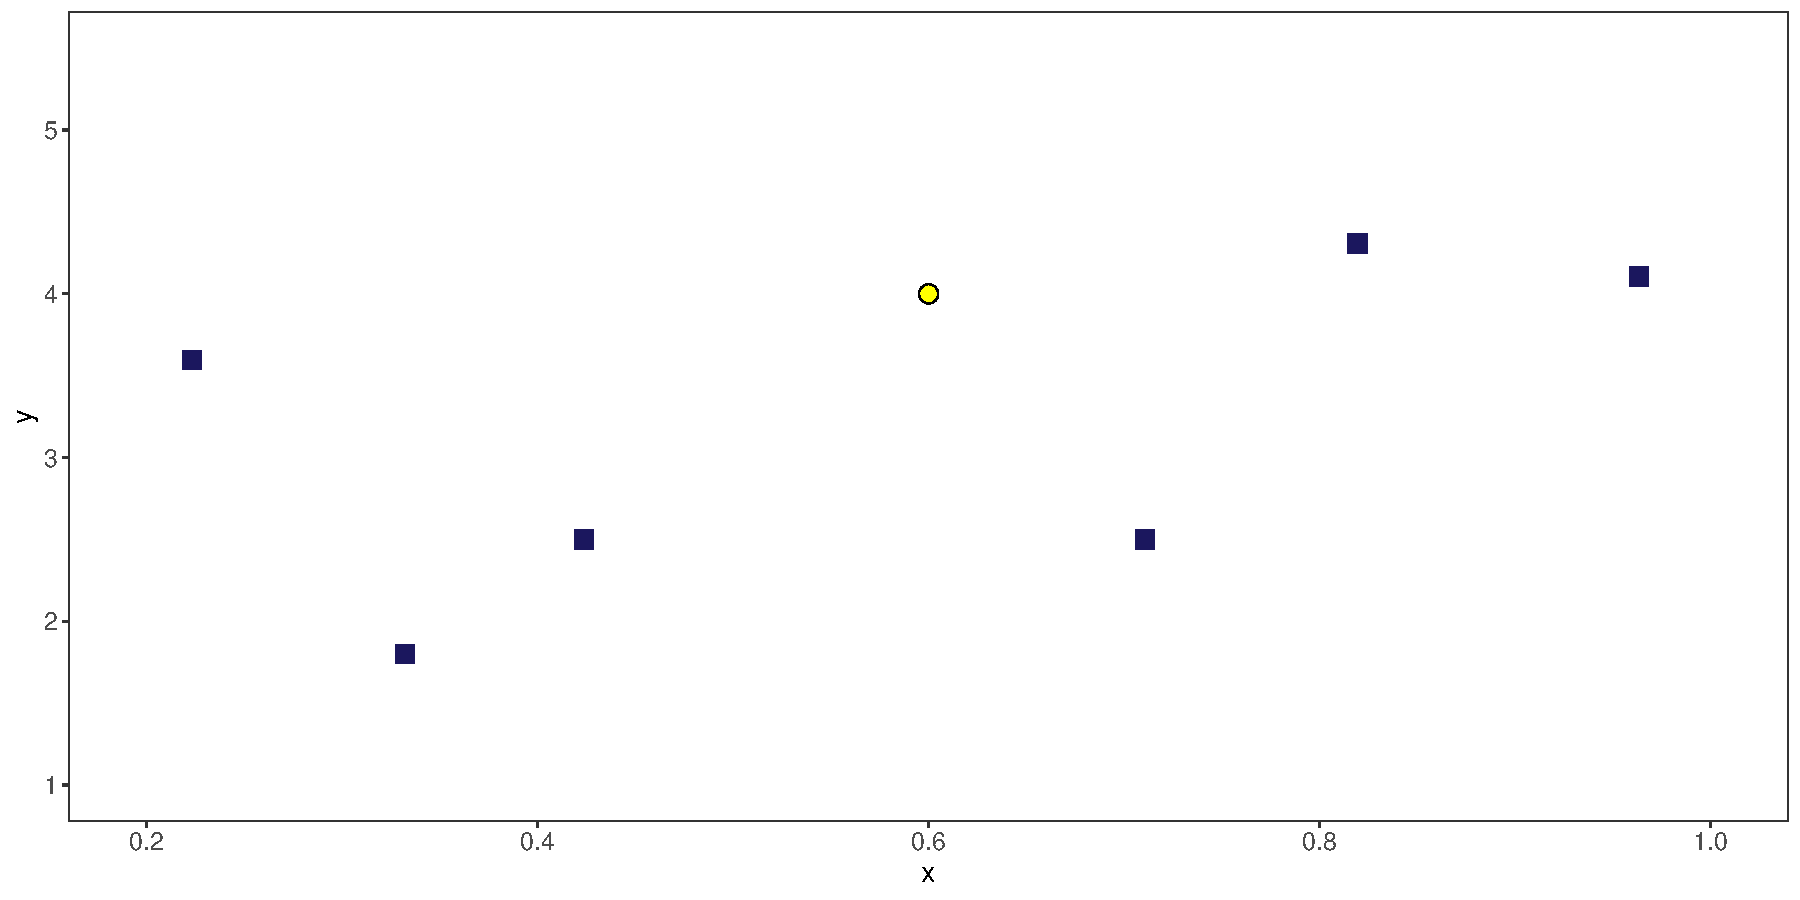
\includegraphics[scale=0.4]{figures/fig_all_sample.pdf}
 \end{figure}

\end{frame}



%----------------------------------------------------------------------%
\begin{frame}[fragile, noframenumbering]
\frametitle{Resampling methods for Out of Sample Prediction}


        \begin{figure}[H] \centering
            \captionsetup{justification=centering}
              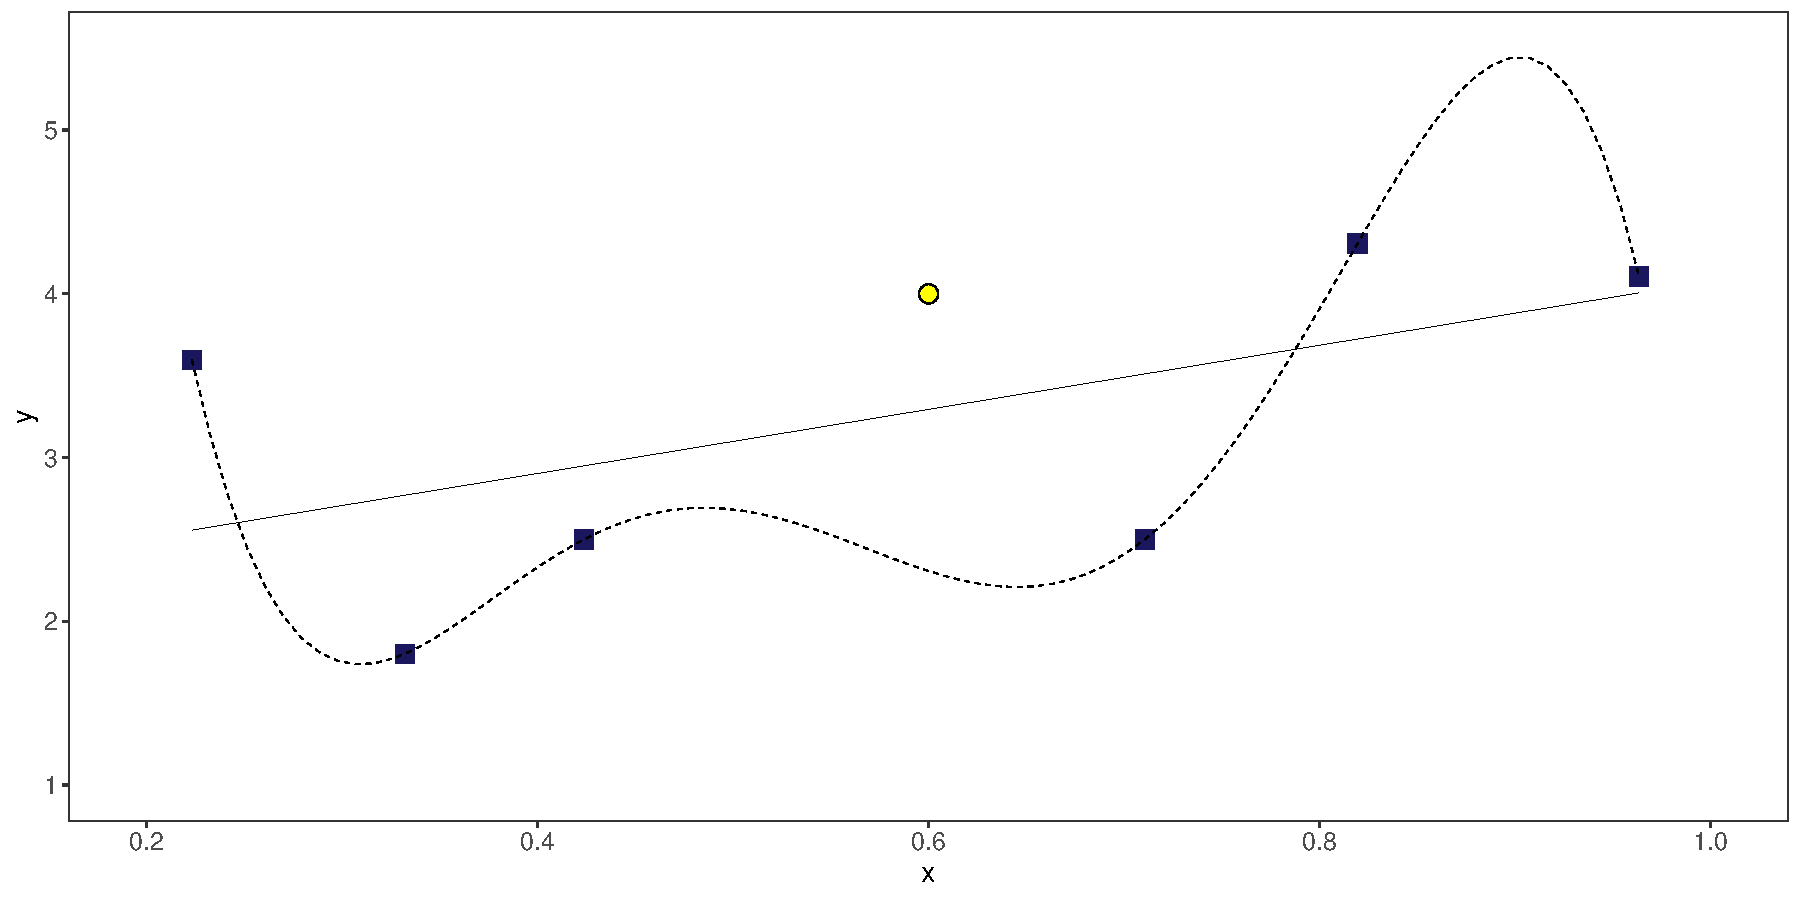
\includegraphics[scale=0.4]{figures/fig_all_sample_polys.pdf}
 \end{figure}


\end{frame}


%----------------------------------------------------------------------%
\begin{frame}<1>[label=pred_error]
\frametitle{Resampling methods for Out of Sample Prediction}


\begin{itemize}
\item Two concepts
\medskip
\begin{itemize}
  \item {\it Test Prediction Error}: is the prediction error in a test sample
  \begin{align}
    Err_{\mathcal{T}est} =E[L(Y,\hat Y)|\mathcal{T}est]
  \end{align}
  \medskip
  \item {\it Training Prediction Error}: is the prediction error in the training sample
  \begin{align}
    Err_{\mathcal{T}rain} =E[L(Y,\hat Y)|\mathcal{T}rain]
  \end{align}
\end{itemize}
\medskip
\pause
  \item Then how do we estimate the test prediction error?
  %\item As the model becomes more and more complex, it uses the training data more and is able to adapt to more complicated underlying structures. 
  %\item Hence there is a decrease in bias but an increase in variance. 
  %\item There is some intermediate model complexity that gives minimum expected test error.
  %\item Unfortunately training error is not a good estimate of the test error
\end{itemize}

\end{frame}




%------------------------------------------------------------------% 

\begin{frame}[fragile, noframenumbering]
\frametitle{Resampling methods for Out of Sample Prediction}

\begin{figure}[H]\centering
           \captionsetup{justification=centering}  
        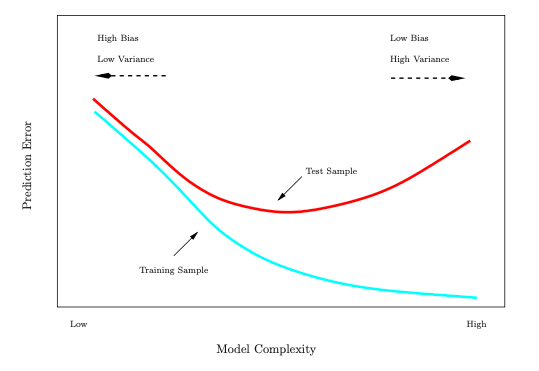
\includegraphics[scale=.6]{figures/train_test_error.png}
    \end{figure}

\end{frame}


%----------------------------------------------------------------------%
%----------------------------------------------------------------------%
\againframe<2>{pred_error}
%------------------------------------------------------------------% 
%------------------------------------------------------------------% 
\begin{frame}[fragile, noframenumbering]
\frametitle{Resampling methods for Out of Sample Prediction}

\begin{itemize}
  \item In the absence of a very large designaed test set we can use some techinques:
  \medskip
  \begin{enumerate}
    \item Validation Set
    \medskip
    \item Loocv
    \medskip
    \item K-fold Crossvalidation
  \end{enumerate}
\end{itemize}

\end{frame}
%------------------------------------------------------------------% 
\begin{frame}[fragile, noframenumbering]
\frametitle{Resampling methods for Out of Sample Prediction}

\begin{figure}[H] \centering
  \centering
  
\includegraphics[scale=0.35]{figures/baticomputer_meme.jpg}
  \\
  \tiny photo from \url{https://www.dailydot.com/parsec/batman-1966-labels-tumblr-twitter-vine/}
\end{figure}

\end{frame}
%----------------------------------------------------------------------%
%----------------------------------------------------------------------%
\end{document}
